%%
%%  Annexes
%%
%%  Note: Ne pas modifier la ligne ci-dessous. / Do not modify the following line.
\ifthenelse{\equal{\Langue}{english}}{
	\addcontentsline{toc}{compteur}{APPENDICES}
}{
	\addcontentsline{toc}{compteur}{ANNEXES}
}
%%
%%
%%  Toutes les annexes doivent être inclues dans ce document
%%  les unes à la suite des autres.
%%  All annexes must be included in this document one after the other.
\Annexe{ARTICLE}
% Texte de l'annexe A\@. Remarquez que la phrase précédente se termine

On inclut à la page suivante l'article \href{https://dl.acm.org/doi/10.1145/3391274.3393637}{\textit{What is the Schema of your Knowledge Graph: Leveraging Knowledge Graph Embeddings and Clustering for Expressive Taxonomy Learning}}, co-écrit avec Amal Zouaq et présenté à la conférence SBD 2020. Son contenu correspond aux chapitres \ref{chap:kge} et \ref{chap:texp} du présent mémoire.
% \textit{International Workshop  on Semantic Big Data} 2020

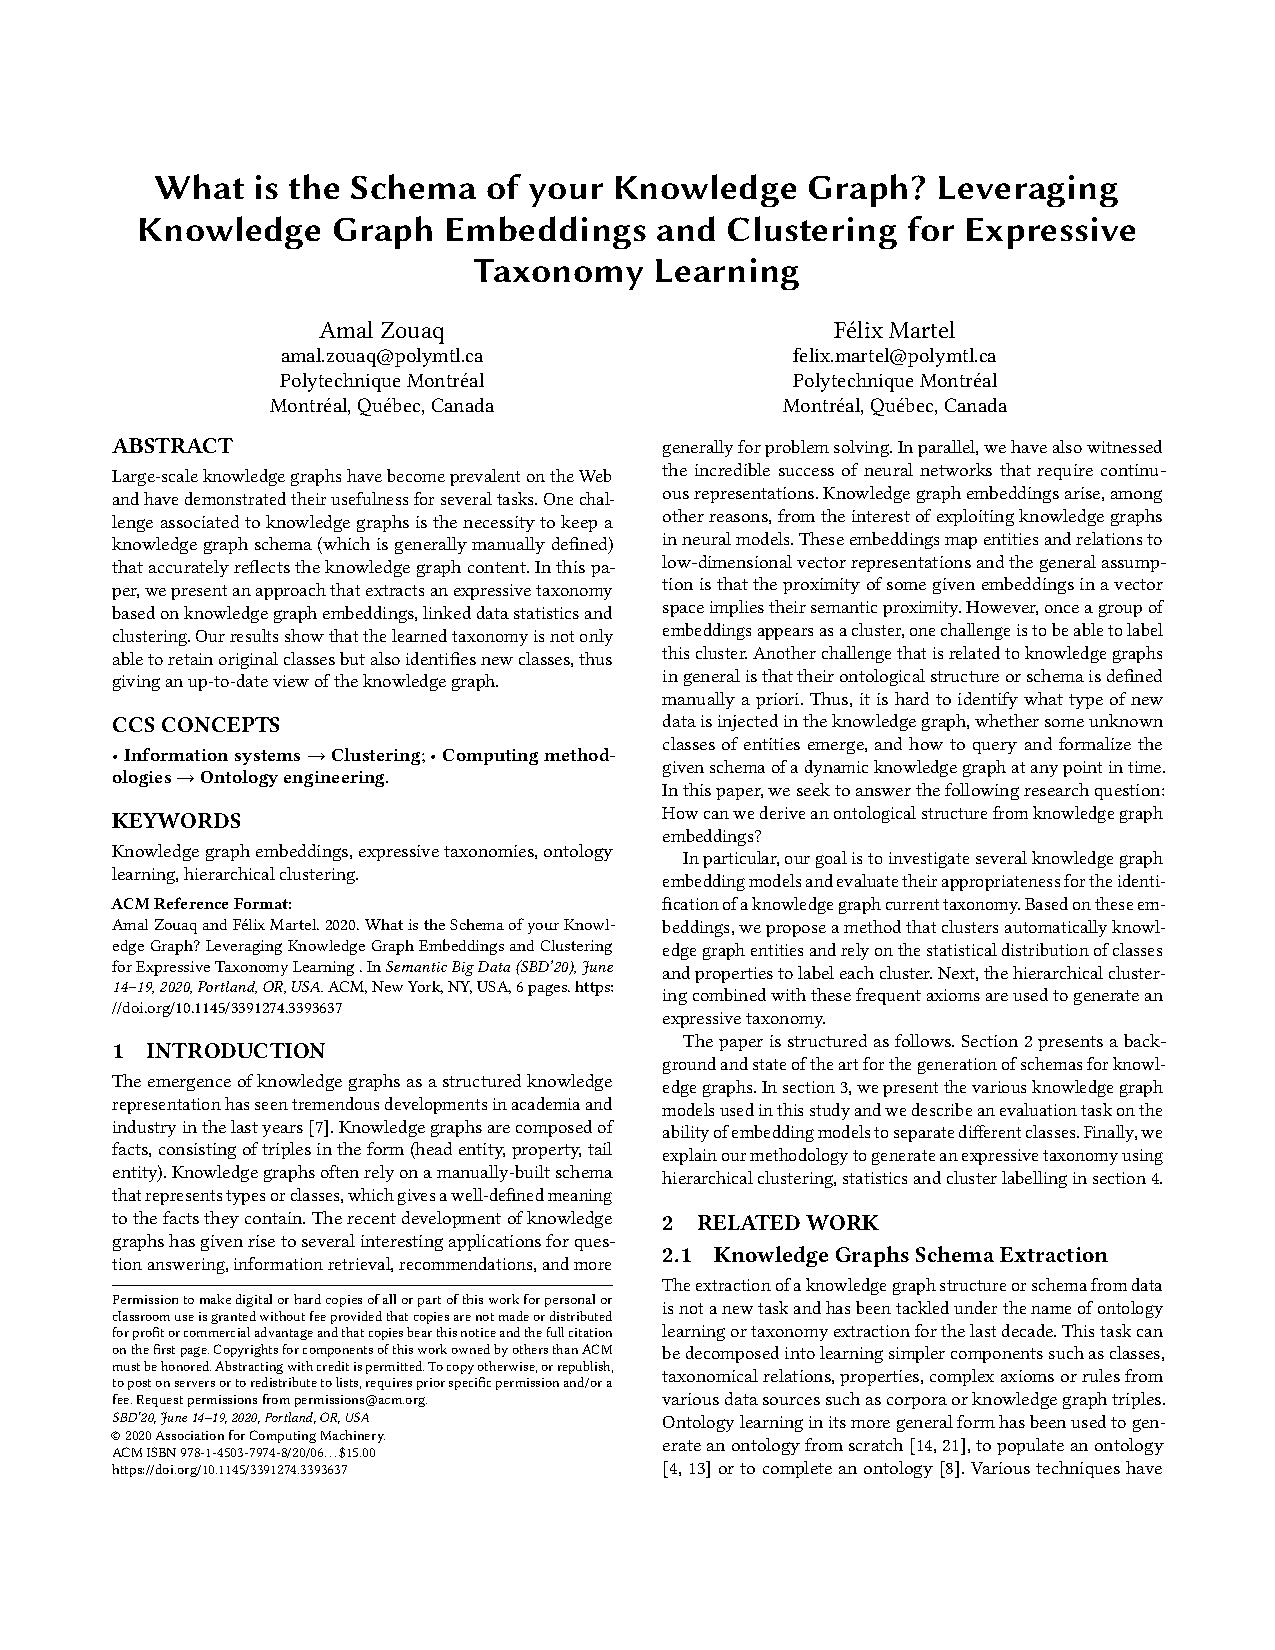
\includepdf[pages=-]{sigmod-article.pdf}
% par une lettre majuscule suivie d'un point. On indique explicitement
% cette situation à \LaTeX{} afin que ce dernier ajuste correctement
% l'espacement entre le point final de la phrase et le début de la
% phrase suivante.
% 
% 
% \begin{landscape}
% \Annexe{Encore une annexe / Another Appendix}
% Texte de l'annexe B\@ en mode «landscape».
% \end{landscape}
% 
% \Annexe{Une dernière annexe / The Last Appendix}
% Texte de l'annexe C\@.


